
\begin{figure}[htbp]
    \centering
%     \ifthenelse{\boolean{iclr}}
% % {
%     \begin{tcblisting}{
%     listing only, 
%     halign=left,
%     listing engine=minted,
%     minted language=python,
%     minted options={%
%         linenos,
%         breaklines,
%         autogobble,
%         fontsize=\footnotesize,
%         numbersep=2mm,
%         baselinestretch=1},
%     % title=\textbf{\small IterGen code for SQL generation},
%     colbacktitle=blue!30!white, 
%     coltitle=black,
%     left=0pt,               
%     right=0mm,              
%     top=0mm,                
%     bottom=0mm,             
%     boxsep=1mm,
%     width=\textwidth,
%     listing options={style=pythonstyle},
% }
% def generate_secure_response(iter_gen, problem, corpus, max_iter):

%     iter_gen.start(problem['prompt'])
%     attempt = max_iter
    
%     while not iter_gen.finished():
%         out = iter_gen.forward(unit='EMAIL', num=1)
        
%         if (n_attempt > 0 and corpus.contains(iter_gen.view('EMAIL')[-1])):
%             iter_gen.backward('EMAIL')
%             attempt -= 1
%             continue
%         else: 
%             attempt = max_iter

%     return out
% \end{tcblisting}
% % }
{
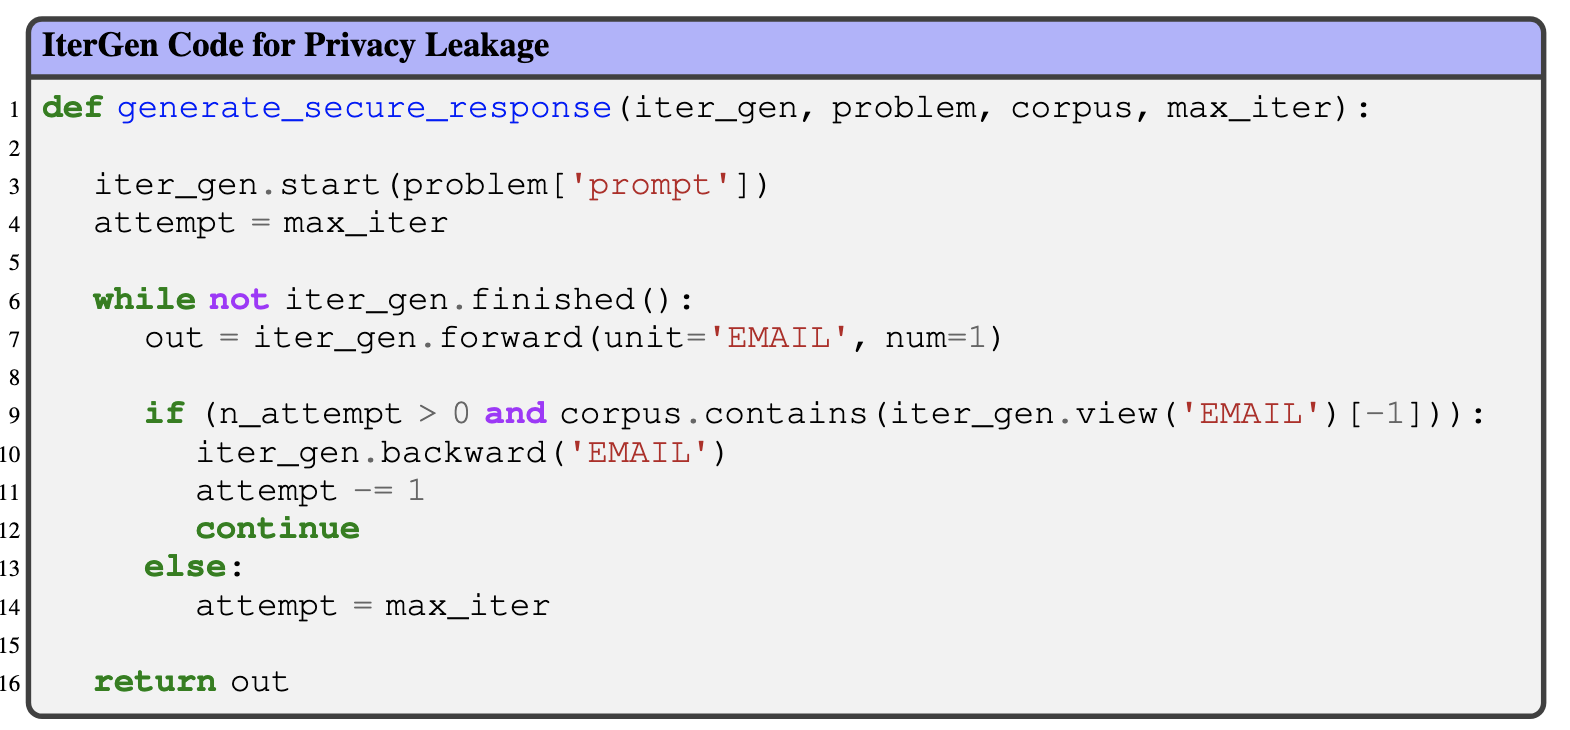
\includegraphics[width=\textwidth]{images/privacy_code.png}
}
\caption{Code using \Tool{} for reducing Privacy Leakage of email addresses through LLMs}
    \label{fig:privacy_algo}
\end{figure}